\chapter{Epsilon Settings}
\label{appendix-epsilon}

The epsilon value settings are traditionally established through conversations between the analyst and decision maker to ensure the trade-off between computation time and a finer-grained search is balanced. Epsilon value settings are also model-specific, as different problems and their model implementations will require different epsilon value configurations, based on the model specification used. As indicated in \cref{step2-moea}, epsilon values used in this study were increased by a factor of 10 from commonly used epsilon values in previous studies involving the lake problem \citep{Quinn2017, Ward2015}. This appendix will explore the impact of the change in epsilon values on the convergence of the MOEA-based search process and on the diversity of the final recommended set of non-dominated policy alternatives. 

The smaller epsilon settings requires significant additional computation time, due to the much larger set of non-dominated alternatives that is discovered and that must be considered each time a new policy is tested to determine whether it is dominated by another policy already in that list. Because of this, epsilon values are compared only for the DPS model variation and MORDM method pairing alone. A comparison of results for the single pairing provides a suitable guideline for the impact of larger epsilon values in all other pairings, especially because each pairing uses the same MOEA for its search. Also due to computational constraints, the smaller epsilon values are tested with 5000 NFE instead of the 100,000 used in the primary study, and only 5 search repetitions were completed (as opposed to the 50 seen in full MORDM runs in this study). 

\begin{figure}[h]
    \centering
    \captionsetup{width=\textwidth}
    
    \begin{subfigure}[b]{\textwidth}
        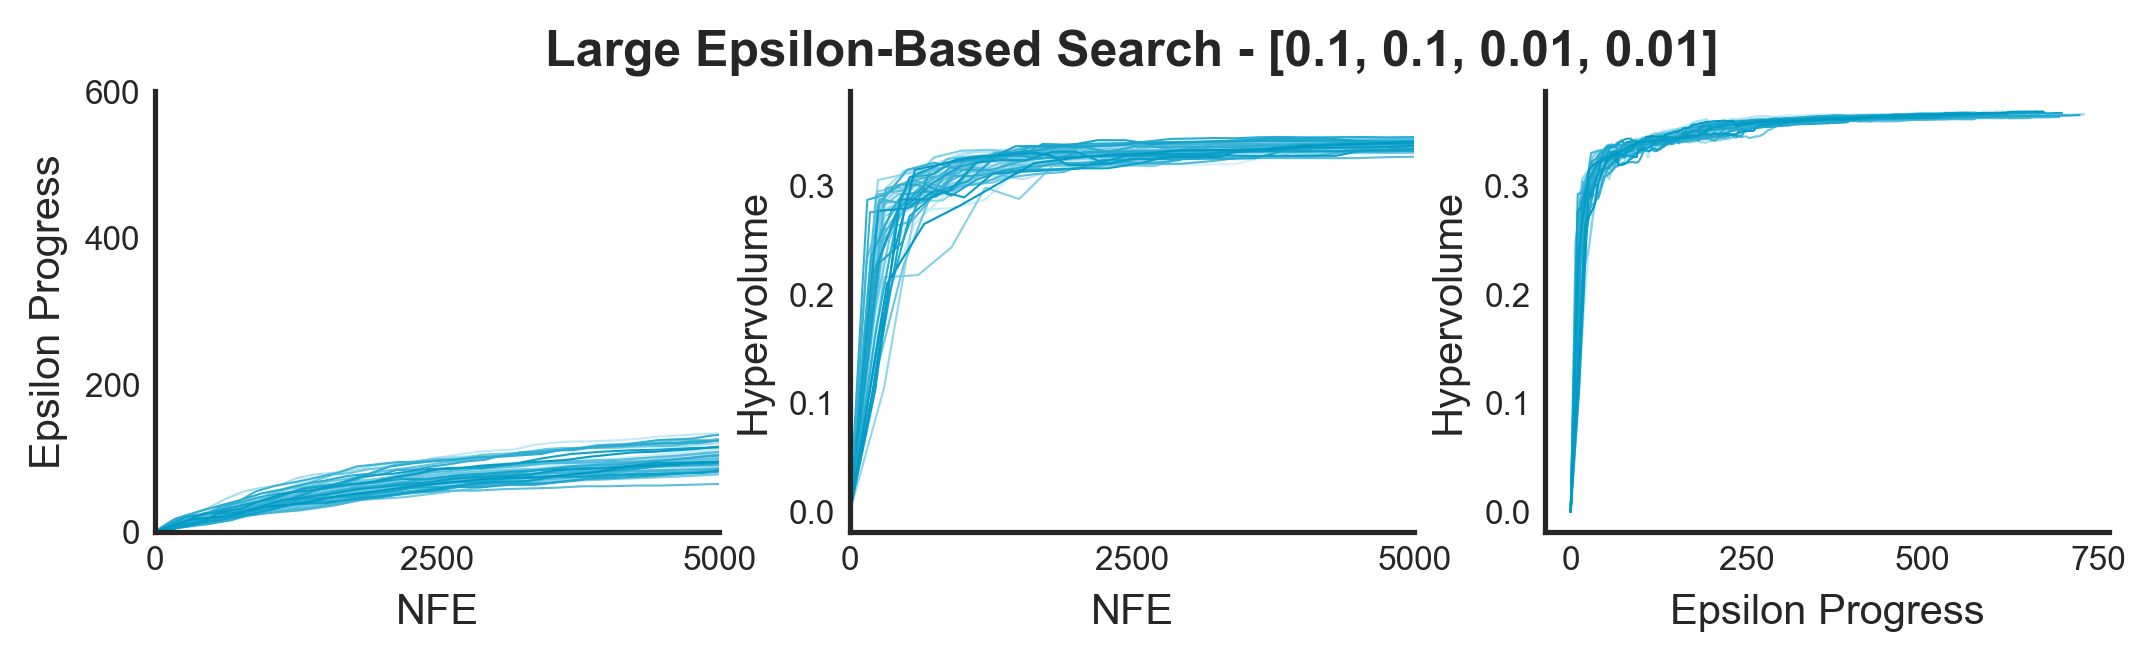
\includegraphics[width=\textwidth]{appendices/epsilon_settings/bigeps_convergence_dps_highres}
        \label{fig:appendix-bigeps}
    \end{subfigure}
    \begin{subfigure}[b]{\textwidth}
        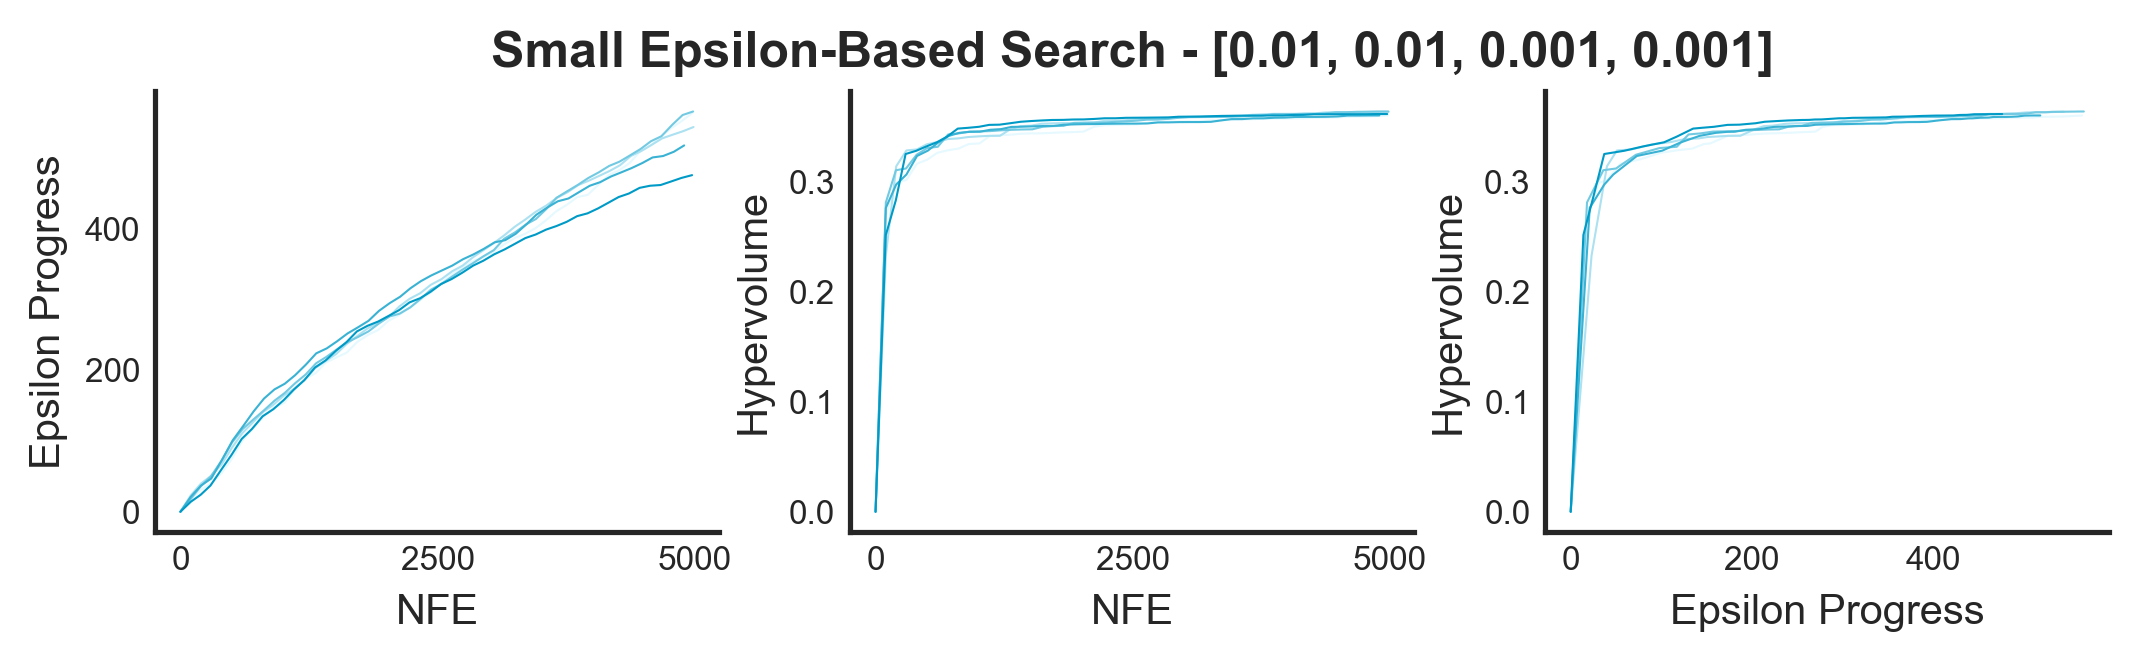
\includegraphics[width=\textwidth]{appendices/epsilon_settings/smalleps_convergence_dps_highres}
        \label{fig:appendix-smalleps}
    \end{subfigure}
    
    \caption[Comparing convergence with different epsilon value settings]{Comparison of the convergence of two MOEA-based searches of the DPS model variation and MORDM pairing using two different epsilon value settings, where the order follows [pollution level, utility, inertia, reliability]. }
    \label{fig:appendix-epsiloncompare}
\end{figure}

\cref{fig:appendix-epsiloncompare} shows the convergence plots for the two sets of epsilon values being compared here. For the sake of the comparison, the number of function executions visible in the case of the large epsilon-based search was limited to 5000, matching the number of function executions used for the small epsilon value. The epsilon progress numbers are quite different between the two settings, with the small epsilon values yielding a much larger epsilon progress value by function execution 5000. This is consistent with the size of epsilon values used in the two sets of charts. As epsilon progress tracks search progress based on the number of policies added to the non-dominated set of alternatives, and because a set of smaller epsilon values will yield a larger number of policies in that set, the epsilon progress should and does increase at a faster rate. 

Hypervolume convergence in \cref{fig:appendix-epsiloncompare}, however, is quite similar between the two settings, both in shape and in value. This indicates that despite significantly different epsilon progress, the sets of non-dominated policy alternatives are covering a similar volume of space within the space described by the set of decision levers and defined in \cref{table:moeaadditional}. 

\begin{table}[h]
    \centering
    \captionsetup{width=0.7\textwidth}
    \caption{Sizes of the non-dominated Pareto front for both small and large epsilon value settings.}
    \label{table:appendix-epsilon-paretosize}
    
    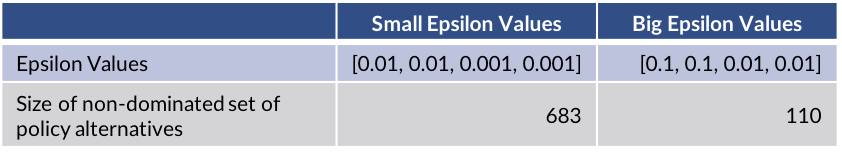
\includegraphics[width=0.7\textwidth]{appendices/epsilon_settings/sizeoffront}
\end{table}

\begin{figure}[h]
    \centering
    \captionsetup{width=\textwidth}
    
    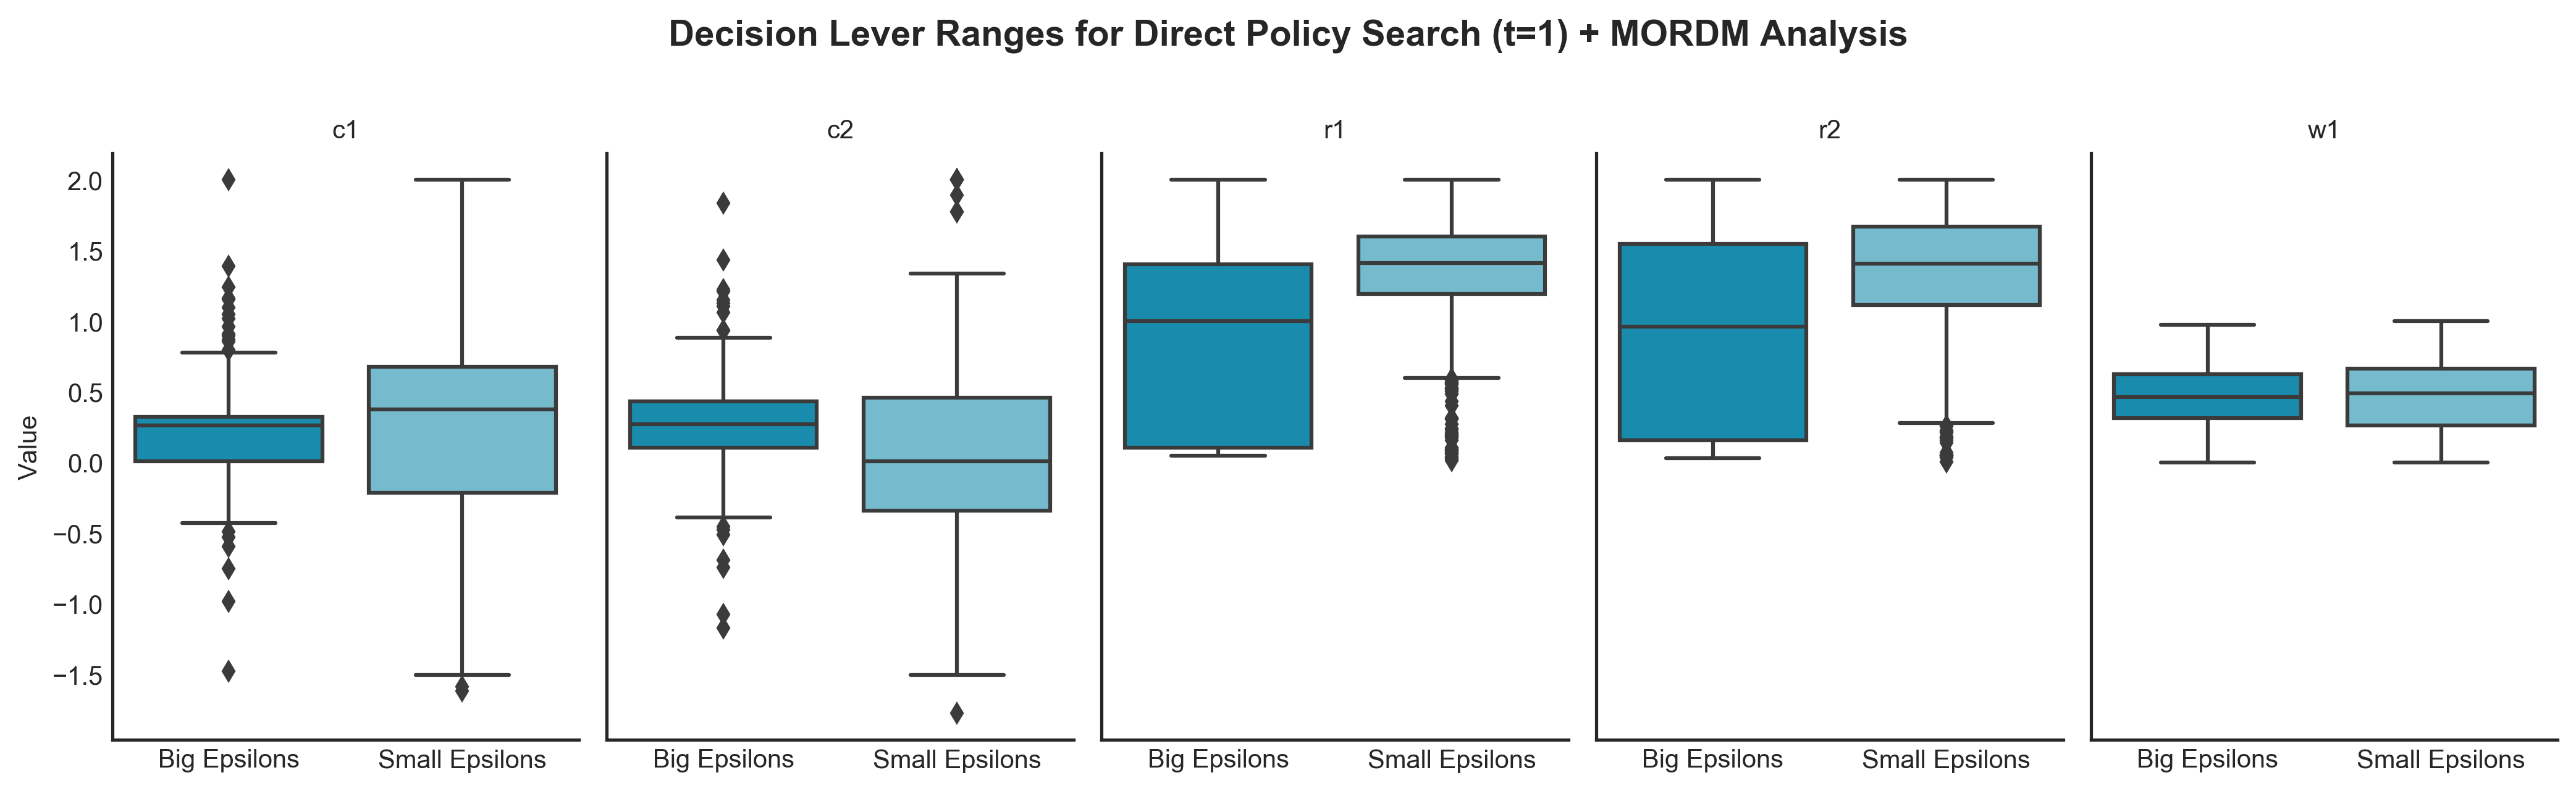
\includegraphics[width=\textwidth]{appendices/epsilon_settings/leverranges_epsilons_box_highres}
    
    \caption[Comparing decision lever values with different epsilon value settings]{Comparison of the ranges of decision lever values between changing epsilon values in the search phase.}
    \label{fig:appendix-epsilondecisionlevers}
\end{figure}

\begin{figure}[h]
    \centering
    \captionsetup{width=0.5\textwidth}
    
    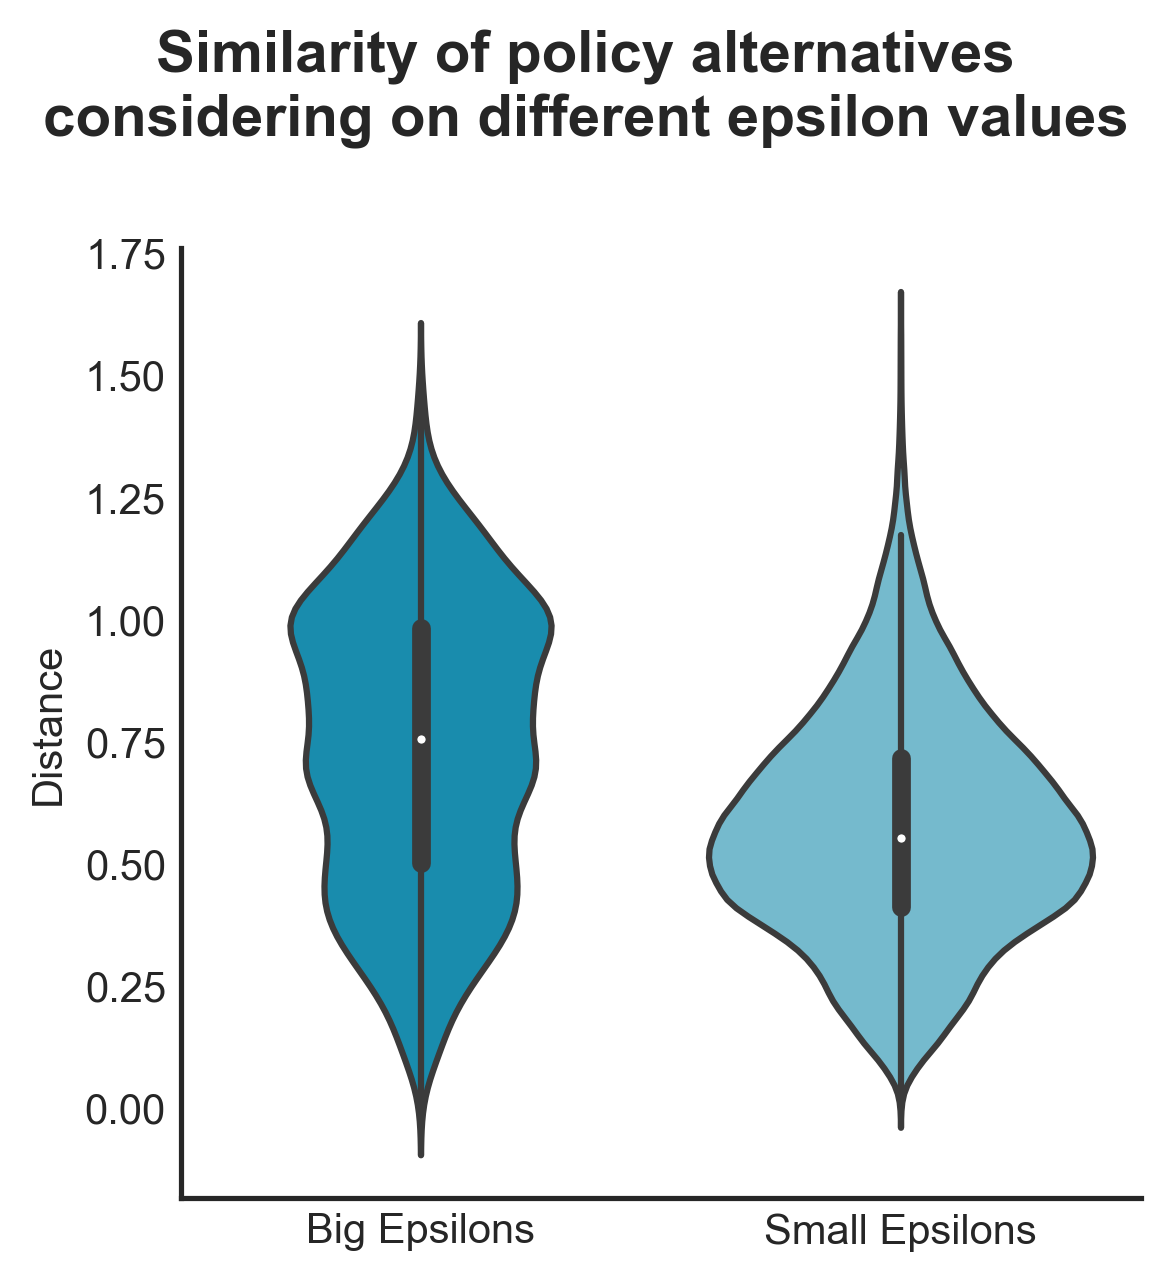
\includegraphics[width=0.3\textwidth]{appendices/epsilon_settings/epsilons_similarity_violin_highres}
    
    \caption[Comparing similarity of alternatives with different epsilon value settings]{Comparison of the similarity of non-dominated policy alternatives for different epsilon settings.}
    \label{fig:appendix-epsilonsimilarity}
\end{figure}

As mentioned earlier, a set of smaller epsilon values will lead to a larger set of non-dominated alternatives, because polices will be included in the set that are closer in value than would be with a set of larger epsilon values. This is borne out in \cref{table:appendix-epsilon-paretosize}, which shows the size of the non-dominated set of policy alternatives for both epsilon value settings. In this case, the number of policy alternatives is over six times larger with smaller epsilon values than seen in this study, which has made use of the larger values. 

The final comparison done is found in \cref{fig:appendix-epsilondecisionlevers}, and \cref{fig:appendix-epsilonsimilarity} which compares the ranges of values for each decision lever of the DPS model variation. Depending on the decision lever, both the larger and smaller epsilon values produce a set of polices with a wider range of values. This indicates that using smaller epsilon values will not necessarily lead to greater diversity of policy alternatives in the case of the lake problem. In fact, \cref{fig:appendix-epsilonsimilarity} seems to confirm that despite the significantly larger size of the non-dominated set of alternatives obtained with smaller epsilon values, the larger epsilon values produce a more diverse set of policy alternatives. It is possible that due to the significantly smaller number of function executions performed with the smaller epsilon values, that the diversity of the set of non-dominated alternatives would have been larger, but these results confirm, at least, that the larger epsilon values are able to produce a set of alternatives with a similar hypervolume and greater diversity than smaller epsilon values would have. Therefore, selecting larger epsilon values should have no negative impact to the results of this study. 

%TODO Also can show robustness changes. EEB


